\documentclass{article}
\usepackage{amsmath}
\usepackage{graphicx}
\usepackage{float}

\title{AP Statistics Part 1 Practice}
\author{Rishi Salwi and Eric Zheng}

\begin{document}
\maketitle

\begin{enumerate}
  % Question 1
  % I'll organize all the plots once they're done
  \item The following plots were created:
    \begin{enumerate}
      \item Stem and leaf plot:
        \begin{figure}[H]
          \centering
          \caption{Stem and Leaf Plot of Women's Heights (in.)}
          \begin{tabular}{r|cccc}
  \hline
  Stem & \multicolumn{4}{l}{Leaf} \\
  \hline
  50. & 2 &   &   &   \\
  51. &   &   &   &   \\
  52. &   &   &   &   \\
  53. & 2 &   &   &   \\
  54. &   &   &   &   \\
  55. &   &   &   &   \\
  56. & 7 &   &   &   \\
  57. & 4 & 9 &   &   \\
  58. & 6 & 9 &   &   \\
  59. & 0 & 3 & 3 &   \\
  60. &   &   &   &   \\
  61. & 4 &   &   &   \\
  62. & 1 & 1 & 4 & 4 \\
  63. & 1 & 1 & 3 &   \\
  64. &   &   &   &   \\
  65. & 4 & 6 &   &   \\
  66. &   &   &   &   \\
  67. & 7 &   &   &   \\
  68. & 5 & 5 &   &   \\
  69. &   &   &   &   \\
  70. & 4 & 5 &   &   \\
  \hline
\end{tabular}

        \end{figure}
      \item Frequency table:
        \begin{table}[H]
          \centering
          \caption{Frequency Table of Women's Heights (in.)}
          \begin{tabular}{c c}
  \hline
  Interval & Frequency \\
  \hline
  $[50.2, 52.7)$ & 1 \\
  $[52.7, 55.2)$ & 1 \\
  $[55.2, 57.7)$ & 2 \\
  $[57.7, 60.2)$ & 6 \\
  $[60.2, 62.7)$ & 5 \\
  $[62.7, 65.2)$ & 3 \\
  $[65.2, 67.7)$ & 2 \\
  $[67.7, 70.2)$ & 3 \\
  $[70.2, 72.7)$ & 2 \\
  \hline
\end{tabular}

        \end{table}
      \item Histogram:
        \begin{figure}[H]
          \centering
          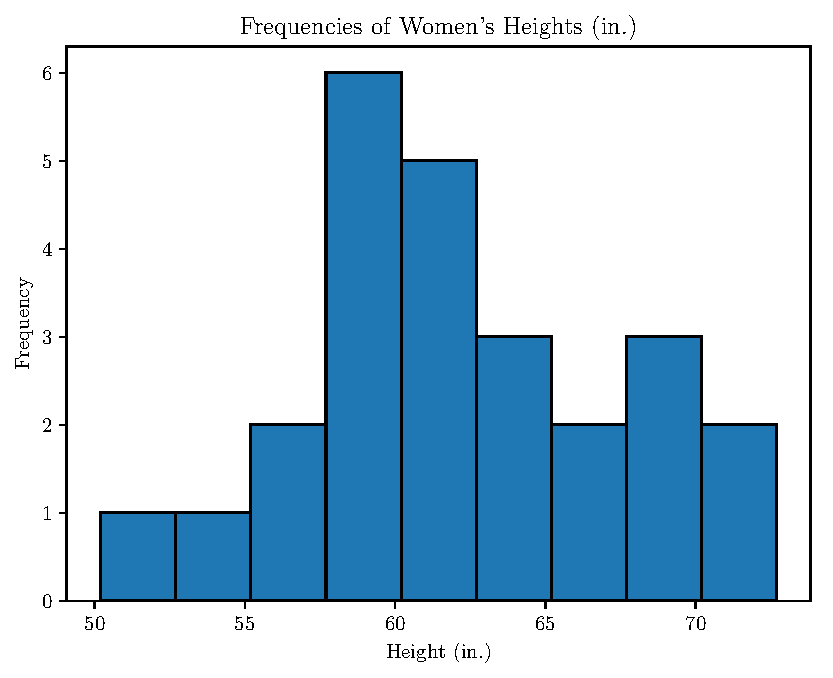
\includegraphics[width=\textwidth]{plots/histogram.pdf}
          \caption{A histogram showing women's heights (in inches)}
        \end{figure}
      \item Pie chart:
        \begin{figure}[H]
          \centering
          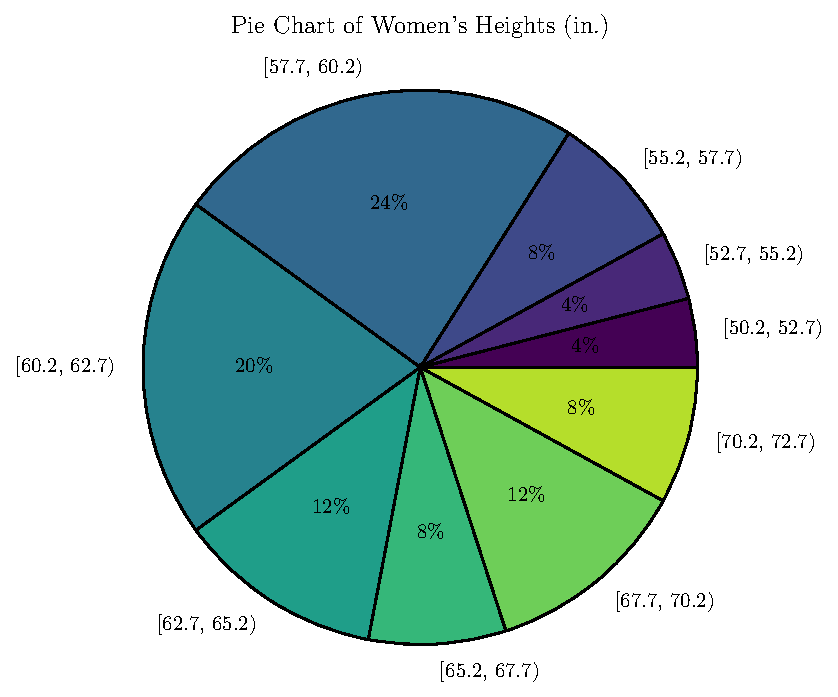
\includegraphics[width=\textwidth]{plots/pie.pdf}
          \caption{A pie chart showing women's heights (in inches)}
        \end{figure}
      \item Box plot:
        \begin{figure}[H]
          \centering
          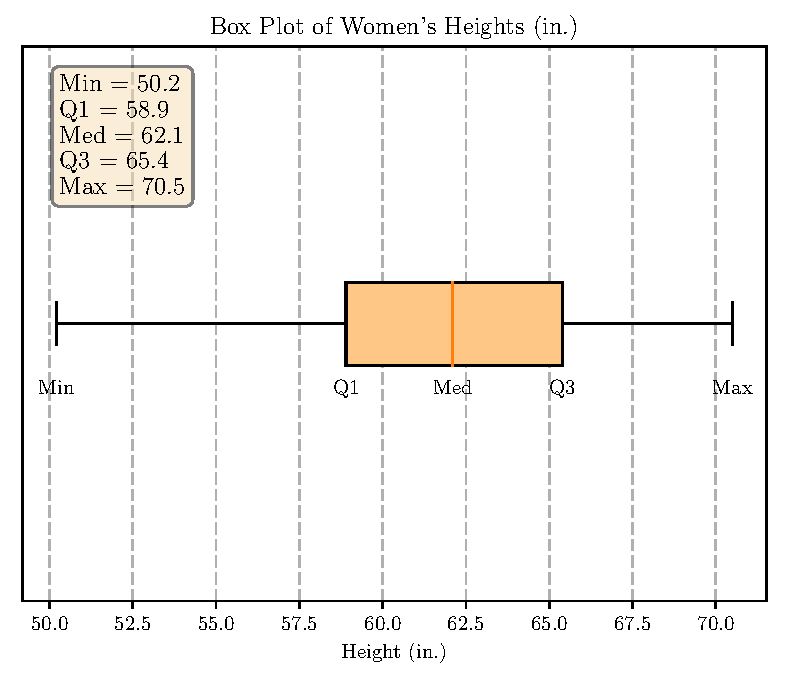
\includegraphics[width=\textwidth]{plots/box.pdf}
          \caption{A box plot showing women's heights (in inches)}
        \end{figure}
    \end{enumerate}

  % Question 2
  \item These data were used to compute the following sample summative statistics:
    \begin{table}[H]
      \centering
      \caption{Summative statistics about women's heights (in inches)}
      \begin{tabular}{l c}
  \hline
  Statistic & Value \\
  \hline
  Mean & 61.88 \\
  Median & 62.1 \\
  Midrange & 60.4 \\
  Mode & 68.5, 63.1, 62.4, 62.1, 59.3 \\
  Range & 20.3 \\
  Standard Deviation & 5.07 \\
  Variance & 25.68 \\
  \hline
\end{tabular}

    \end{table}

  % Question 3
  \item The data set is not normally distributed; this can be most easily seen from the shape of the histogram, which does not resemble a bell curve. It is not symmetric because it is skewed to the left. I know this because there is a whale tail.
\end{enumerate}
\end{document}
